\section{Results}
\label{sec:dialects-results}

The results section is structured as follows:
I first present the performance of the model and general information on the LIME-based importance scores in \autoref{sec:dialects-results-general}.
I then focus on the top 50 features per dialect group and analyze to what extent they reflect the linguistic features that are traditionally considered the most important distinctive features in Norwegian dialectology (\autoref{sec:dialects-results-lingmajor}) and other linguistics features (\autoref{sec:dialects-results-lingother}).

\subsection{General observations}
\label{sec:dialects-results-general}

I train and test the dialect classification model in ten initializations, each on a different train-test split of the dataset, and extract LIME importance scores from each of these runs.
All of the scores in this section are mean values across all ten runs.
The average model accuracy is 78.6~\% and the average (macro-averaged) F$_1$~score is 77.1~\%.

\begin{figure}[htbp]
    \centering
    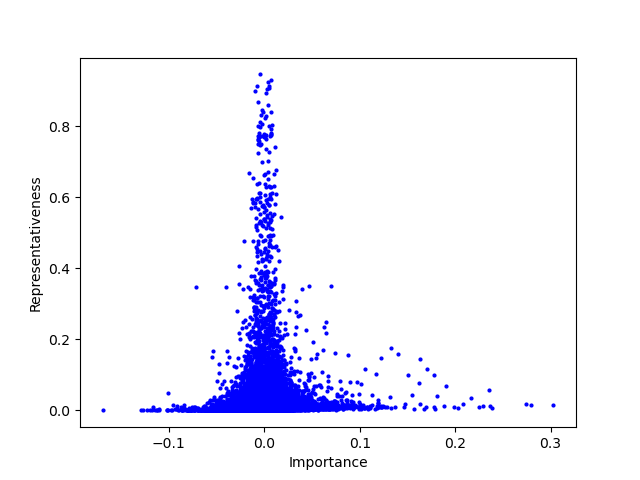
\includegraphics[width=0.9\textwidth]{figures/3-dialects/importance-rep-all-mean-unscaled.png}
    \caption
    [Representativeness values by LIME score for dialect classification]
    {Representativeness values by LIME importance score per feature-label combination.}
    \label{fig:imp-rep}
\end{figure}
\begin{figure}[htbp]
    \centering
    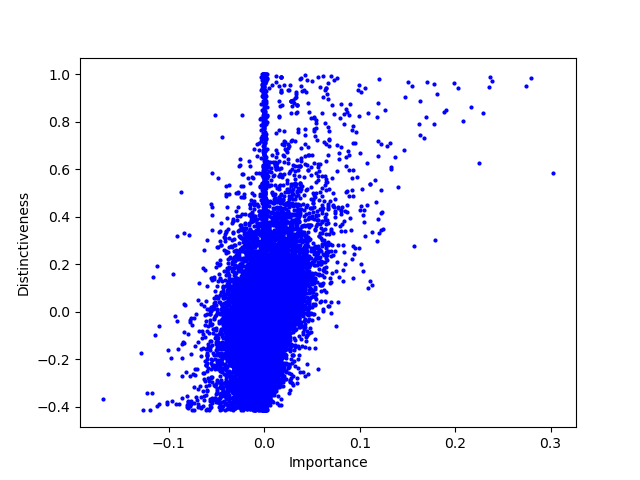
\includegraphics[width=0.9\textwidth]{figures/3-dialects/importance-dist-all-mean-unscaled.png}
    \caption
    [Distinctiveness values by LIME score for dialect classification]
    {Distinctiveness values by LIME importance score per feature-label combination.}
    \label{fig:imp-dist}
\end{figure}

Importance values range between -0.17 and +0.30, with no significant distribution differences for the different dialect groups.
There is only a marginal correlation between a feature's importance score for a label and the corresponding representativeness value, i.e. in which proportion of the instances with that label it is present.
This is not very surprising, as most features with high representativeness scores are representative of \textit{all} dialect groups.
This is for instance the case with almost all character unigrams.
The correlation coefficient (Pearson's \textit{R}) between importance and representativeness is between 0.03 and 0.05 for the different dialect groups,
and this is also illustrated in \autoref{fig:imp-rep}.
However, the importance score does correlate with the distinctiveness score, that is, features with higher importance scores for a label tend to mostly occur in utterances with that gold-standard label (\autoref{fig:imp-dist}).
The correlation coefficient between importance and distinctiveness is between 0.37 and 0.41 for the different dialect groups.


\begin{table}[htbp]
    \centering
\begin{tabular}{lrlrlrlrl}
\toprule
\textbf{Word} & \multicolumn{2}{l}{\begin{tabular}[c]{@{}l@{}}\textbf{West} (actual\\\& predicted label)\end{tabular}} & \multicolumn{2}{l}{\textbf{East}} & \multicolumn{2}{l}{\textbf{Trønder}} & \multicolumn{2}{l}{\textbf{North}} \\
\midrule
\textit{ja} /ja/ {\smaller``yes''}  &  & &  &  &  &  &  &  \\
\multirow{2}{*}{\begin{tabular}[c]{@{}l@{}}\textit{da} /då/ \\ \phantom{~~}{\smaller``then''} \end{tabular}} & \cellcolor[HTML]{72C69D}0.17  & då\sep{}& {\cellcolor[HTML]{F5CDCA}-0.07} & då\sep{} & {\cellcolor[HTML]{F5CECB}-0.07} & \multicolumn{2}{l}{då\sep{}}  &  \\
 & \cellcolor[HTML]{F7D6D3}-0.06 & \sep{}då &  &  &  &  &  &  \\
\textit{vi} /me/ {\smaller``we''} & \cellcolor[HTML]{A1D9BE}0.11  & \multicolumn{2}{l}{{\ngram{\sos{}vi/me\eos{}}}}  &  &  &  & {\cellcolor[HTML]{F5CBC7}-0.08} & {\ngram{\sos{}vi/me\eos{}}}  \\
\multirow{2}{*}{\begin{tabular}[c]{@{}l@{}}\textit{har} /he/\\ \phantom{~~}{\smaller``have.\textsc{pres}''} \end{tabular}} & \cellcolor[HTML]{BAE3CF}0.08 & he\sep{} & {\cellcolor[HTML]{F7D6D4}-0.06} & he\sep{} &  &  &  &  \\
 & \cellcolor[HTML]{D2EDE0}0.05 & \multicolumn{2}{l}{\sos{}har/he\eos{}} &  &  &  &  &  \\
\multirow{2}{*}{\begin{tabular}[c]{@{}l@{}}\textit{de} /di/ \\ \phantom{~~} {\smaller``the.\textsc{pl}''} \end{tabular}}& \cellcolor[HTML]{D1EDDF}0.06  & \sep{}di&  &  &  &  &  &  \\
\\
\multicolumn{3}{l}{\textit{siste} /sisste/ {\smaller``last.\textsc{def}''}}  & &  &  &  &  &  \\
\multicolumn{3}{l}{\textit{årene} /åran/ {\smaller``years.\textsc{def}''}}  & &  &  &  &  &  \\
\multirow{2}{*}{\begin{tabular}[c]{@{}l@{}}\textit{nå} /nå/\\ \phantom{~~}{\smaller``now''} \end{tabular}}& \cellcolor[HTML]{F1B7B3}-0.11 &  \sep{}nå & &  &  &  &  &  \\
 & \cellcolor[HTML]{BFE5D2}0.08 & nå\sep{} &  &  &  &  &  &  \\
\textit{så} /så/ {\smaller``so''} &  & &  &  &  &  &  &  \\
\multirow{2}{*}{\begin{tabular}[c]{@{}l@{}}\textit{har} /he/\\ \phantom{~~}{\smaller``have.\textsc{pres}''} \end{tabular}} &  \cellcolor[HTML]{D2EDE0}0.05 &\multicolumn{2}{l}{\sos{}har/he\eos{}}  &  &  &  &  &  \\
 & \cellcolor[HTML]{BAE3CF}0.08 & he\sep{} &  &  &  &  &  &  \\
\textit{vi} /mi/ {\smaller``we''} & \cellcolor[HTML]{94D4B5}0.13 & {\smaller\ngram{\sos{}vi/mi\eos{}}} & {\cellcolor[HTML]{F7D9D7}-0.06}& \multicolumn{3}{l}{{\ngram{\sos{}vi/mi\eos{}}}}  & {\cellcolor[HTML]{F7D5D3}-0.06}& {\ngram{\sos{}vi/mi\eos{}}}  \\
& \cellcolor[HTML]{AFDFC8}0.10  & \sep{}mi &  {\cellcolor[HTML]{F4C7C3}-0.09} &\sep{}mi &  &  &  &  \\
\multicolumn{3}{l}{\textit{vært} /værrt/ {\smaller``been''}} &  &  &  &  &  &  \\
\multicolumn{3}{l}{\textit{heldige} /helldi/ {\smaller``lucky.\textsc{pl}''}}  & &  &  &  &  &  \\
\bottomrule
\end{tabular}
    \caption
    [LIME scores for a sample utterance]
    {LIME scores for a (correctly predicted) West Norwegian utterance.
    Features with importance scores between -0.05 and +0.05 are omitted to preserve space.
    No word bigrams have importance scores that lie below/above that threshold.}
    \label{tab:sample-sentence}
\end{table}

\autoref{tab:sample-sentence} shows the importance scores for each label for a sample sentence, the West Norwegian utterance \textit{ja da [.] vi har [---] de siste årene nå så har vi vært heldige}
/ja då me he di sisste åran nå så he mi værrt helldi/
``Yes. We have---the past few years now, we've been lucky.''
(Note that these are the LIME scores for this specific utterance and not the global importance scores.)
This utterance is represented by 100 features, the vast majority of which have LIME scores that are close to zero.
This utterance was correctly predicted as West Norwegian and that prediction is also reflected by the distribution of importance scores: in this case, only the West Norwegian label is associated with (more than marginally) positive importance scores, while the importance scores for the other combinations of features and labels tend to be close to zero (signifying that a feature is insignificant for predicting the given label) or negative (indicating that the presence of the feature lowers the likelihood of the given label being predicted).
It should be noted that importance scores can seem contradictory: in the sample sentence, the words \textit{da} /d\aa/ and \textit{n\aa} /n\aa/ are represented by a feature \ngram{\sep{}d\aa} (\ngram{\sep{}n\aa}) ``/d\aa/ (/n\aa/) is a prefix (or full word)'' and another feature \ngram{d\aa\sep{}} (\ngram{d\aa\sep{}}) ``/d\aa/ (/n\aa/) is a suffix (or full word),'' where the former receives a negative importance score and the latter a positive one.


\begin{figure}[htbp]
    \centering
    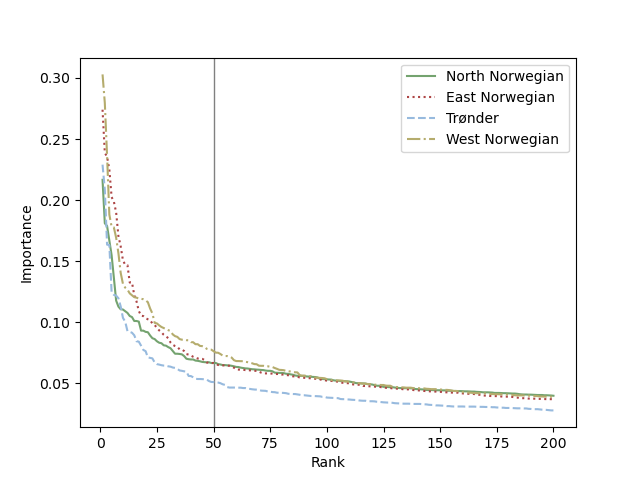
\includegraphics[width=0.9\textwidth]{figures/3-dialects/importance-rank-all-mean-unscaled-50.png}
    \caption
    [Importance score by rank and dialect group]
    {Importance score by rank and dialect group.}
    \label{fig:imp-rank}
\end{figure}
\begin{figure}[htbp]
    \centering
    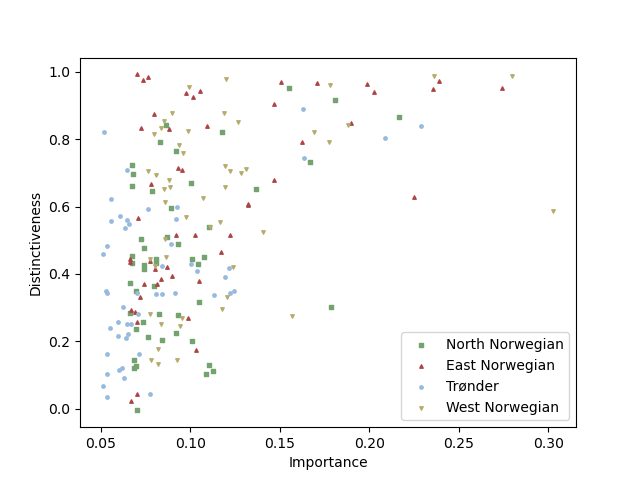
\includegraphics[width=0.9\textwidth]{figures/3-dialects/importance-dist-all-mean-unscaled-50.png}
    \caption[Distinctiveness by LIME score for the 50 highest-ranking features per dialect group]
    {Distinctiveness by importance score for the 50 highest-ranking features per label.}
    \label{fig:imp-dist50}
\end{figure}

In the following two sections, I qualitatively examine the 50 features with the highest importance scores per predicted label.
I chose this threshold to strike a balance between only analyzing features with relatively high importance scores and having a sizable selection of features to analyze.
\autoref{fig:imp-rank} shows the importance scores for the features included in the analysis as well as the scores of the succeeding ranks.
The selected features show a correlation between importance score and distinctiveness, as illustrated in \autoref{fig:imp-dist50}.
The following analysis includes the 50 features per class that have the highest importance scores.\footnote{%
I share tables with the 200 most important features per dialect group at \url{https://github.com/verenablaschke/ma-thesis/tree/main/models/dialects}.
}
These features tend to mostly include variants of high-frequency words, as well as some common short sequences of phonemes.
Only one of those high-importance features is clearly about a conversation topic (rather than lexical choice or pronunciation): the trigram \ngram{ami} in North Norwegian utterances, which usually appears in the word \textit{samisk} `Sámi' and inflected versions thereof.
This is not a surprise as most Sámi cultural centres are located in the Northern part of the country.



